\chapter{Regular Languages}

\section{Finite Automata}
Finite automata is a model for a computer with an extremely  limited amount of memory. For instance, consider a controller for an automatic door. We can have two states, open or closed. And 4 input conditions, front, rear, neither and both. 

\vspace{1em}

\begin{definition}
    A \textbf{\emph{finite automaton}} is a 5-tuple ($Q,  \Sigma, \delta, q_{0}, F$) where, 
    \begin{enumerate}
        \item $Q$ is a finite set called the states
        \item $\Sigma$ is a finite set called the alphabet
        \item $\delta : Q \times \Sigma \to Q$ is the transition function
        \item $q_{0} \in Q$ is the start state
        \item $F \subseteq Q$ is the set of accept states.
    \end{enumerate}
\end{definition}
\begin{remark}
    By this definition we can have $\emptyset \subseteq Q$ and hence have no accept states.
\end{remark}
\begin{note}
Note also that $\delta$ a function defined from the domain $Q \times \Sigma$ and hence every state has a transition to another state for any given input alphabet.
\end{note}


Consider the following autoamta $M_{1}$, 
\begin{enumerate}
    \item $Q = \{q_{1}, q_{2}, q_{3}\}$
    \item $\Sigma = \{0, 1\}$
    \item $\delta$ is, 
    \[
        \begin{tabular}{c|c c}
             & 0  & 1\\
            \hline
            q_{1} & q_{1} & q_{2}\\
            q_{2} & q_{3} & q_{2}\\
            q_{3} & q_{2} & q_{2}\\
        \end{tabular}
    \]

    \item $q_{1}$ is the start state
    \item $F = \{q_{2}\}$
\end{enumerate}

Now let $A$ be the set of all strings that our machine accepts, then we say that $A$ is the language of machine $M$  and $L(M) = A$.

\vspace{1em}

In this case if we have, 
\[
    A = \{w \mid w \text{ contains at least one $1$ and an even number of $0s$ follow the last $1$ }\}
\]

Then we have $M$ recognizes $A$.
\begin{note}
    Note that even number of zeros also means zero zeroes and hence we can have the string end with just $1$.
\end{note}

\subsection{Computation}
Let $M$ be a finite automata (with the usual 5-tuple representation). Let $w = w_{1}w_{2}\dots w_n$ be a string where each $w_i$ is a member of $\Sigma$. We say $M$ accepts $w$ if there exists a sequence of states $r_{0}, \dots, r_n$ in $Q$ such that, 
\begin{enumerate}
    \item $r_{0} = q_{0}$
    \item $\delta(r_i, w_{i + 1}) = r_{i + 1}$, for $i = 0, \dots, n - 1$
    \item $r_n \in F$
\end{enumerate}
\begin{remark}
    Condition 1 says that we start in the start state. Condition 2 says that we transition according to our string and Condition 3 states that we end with a accept state.
\end{remark}

\begin{definition}
    A language is called a \textbf{\emph{regular language}} if a finite automata recognizes it. 
\end{definition}

\subsection{Regular Operations}
\begin{definition}
Let $A, B$ be langauges. We define the regular operations $\textbf{union, concatenation} \\
\textbf{ and star} $ as follows, 
    \begin{enumerate}
        \item Union: $A \cup B = \{x \mid x \in A \text{ or } x \in B\}$
        \item $A \circ B = \{xy \mid x \in A \text{ and } y \in B\}$
        \item $A^{*} = \{x_{1}\dots x_k \mid k \ge 0 \text{ and each }x_i \in A\}$
    \end{enumerate}
\end{definition}
\begin{eg}
    If $\Sigma$ is the regular alphabet and $A = \{good, bad\}$ and $B = \{boy, girl\}$ then,
    \begin{itemize}
        \item $A \cup B = \{good, bad, boy, girl\}$
        \item $A \circ B = \{goodboy, goodgirl, badboy, badgirl\} $
        \item $A^{*} = \{\epsilon, good, bad, goodgood, goodbad, badgood, badbad, goodgoodgood,\\goodgoodbad,goodbadgood,goodbadbad, \dots\}$
    \end{itemize}
\end{eg}


\begin{theorem}
    The class of regular languages is closed under the union operation.
\end{theorem}
\begin{note}
    This means that if $A_{1}$ and $A_{2}$ are regular languages then so is $A_{1} \cup A_{2}$
\end{note}
\begin{proof}
    If $A_{1}$ is regular there exists a finite automaton $M_{1}$ that accepts it. Similarly we have $M_{2}$. Now the goal is to construct a new finite automaton $M$ that can accept both languages. We can do this by having $M$ simulate both $M_{1}$ and $M_{2}$. Define $M = \{Q, \Sigma, \delta, q_{0}, F\}$ as follows, 
    \begin{enumerate}
        \item $Q = \{(r_{1}, r_{2}) \mid r_{1} \in Q_{1} \text{ and } r_{2} \in Q_{2}\}$
        \item $\Sigma$ is the same as both $M_{1}$ and $M_{2}$ (the union of both their alphabets if $M_{1}, M_{2}$ differ in their alphabet)
        \item $\delta$ is defined from $(Q_{1} \times Q_{2}) \times \Sigma \to (Q_{1} \times Q_{2})$ as follows for $(r_{1}, r_{2}) \in Q$ we have,
        \[
            \delta((r_{1}, r_{2}), a) = (\delta_{1}(r_{1}, a), \delta_2(r_{2}, a))
        \]

    \item $q_{0}$ is the pair $(q_{1}, q_{2})$
    \item $F = \{(r_i, r_j) \mid r_i \in F_{1} \text{ or } r_{j} \in F_{2}\}$
    \end{enumerate}
\end{proof}

\begin{theorem}
    Regular languages are closed under concatenation
\end{theorem}
\begin{proof}
    Consider we have two regular languages $A_{1}, A_{2}$ corresponding to $M_{1}$ and $M_{2}$. We need a new finite automata $M$ that is able to accept the concatenation of languages from $A_{1}$ and $A_{2}$. So essentially from every accept state of $M_{1}$ once the string from $A_{1}$ is finishes we need a mechanism to switch to $M_{2}$ in order to compute the string from $A_{2}$. This means that from the accept states we might have multiple arrows for the same alphabet. 

    \vspace{1em}
    
    To allow this, we need to introduce a new concept called \textbf{nondeterminism}.
\end{proof}

\section{Nondeterminism}
When a machine is in a given state and reads the next input symbol, if the next state is predetermined (i.e only a single choice is there) then we called it a deterministic computation. In a nondeterministic machine, several choices may exists for the next state at any point.

\vspace{1em}

This is a generalisation of a deterministic machine (so every determinstic finite automaton is a non deterministic finite automaton).



\begin{figure}[h]
  \centering
  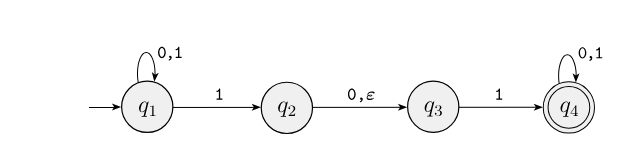
\includegraphics[width=0.8\textwidth]{assets/nondeterministic-finite-automaton.png}
  \caption{Nondeterministic finite automaton}
  \label{fig:nondeterministic-finite-automaton}
\end{figure}


Clearly a deterministic finite automata  has only one arrow for each symbol in our alphabet but a non-deterministic can have \textbf{zero, one or more}. In addition to symbols of our alphabet we can also have arrows with the label $\epsilon$ which mean a lack 
